% 18 variables in here:
% h_1 = 10.0, h_2 = 10.0, h_3 = 10.0, h_4 = 10.0, h_5 = 10.0, h_6 = 10.0, ux_1 = 0.0, ux_2 = 0.0, ux_3 = 0.0, ux_4 = 0.0, ux_5 = 0.0, ux_6 = 0.0, uy_1 = 0.0, uy_2 = 0.0, uy_3 = 0.0, uy_4 = 0.0, uy_5 = 0.0, uy_6 = 0.0
\begin{figure}[h!]
\centering
  \subfigure[1st basis function, $x$-momentum] {
    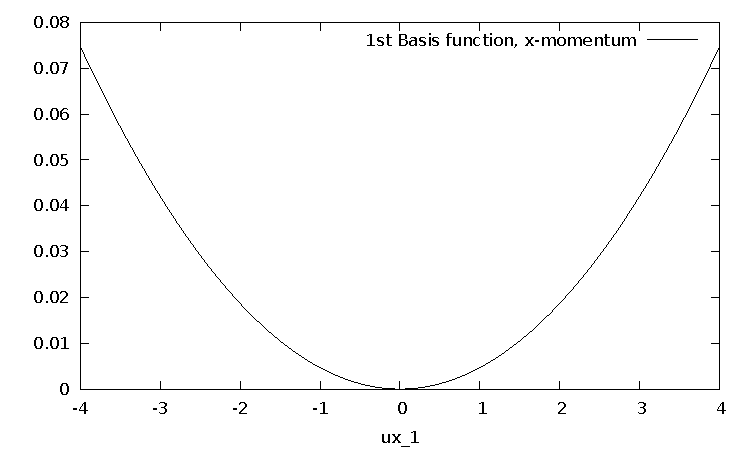
\includegraphics[scale=\zoomfactor]{{{ord2_varying_ux_1/10.0_10.0_10.0_10.0_10.0_10.0_y_0.0_0.0_0.0_0.0_0.0_0.0_0.0_0.0_0.0_0.0_0.0f00}}}
  }
  % \subfigure[] {
  %   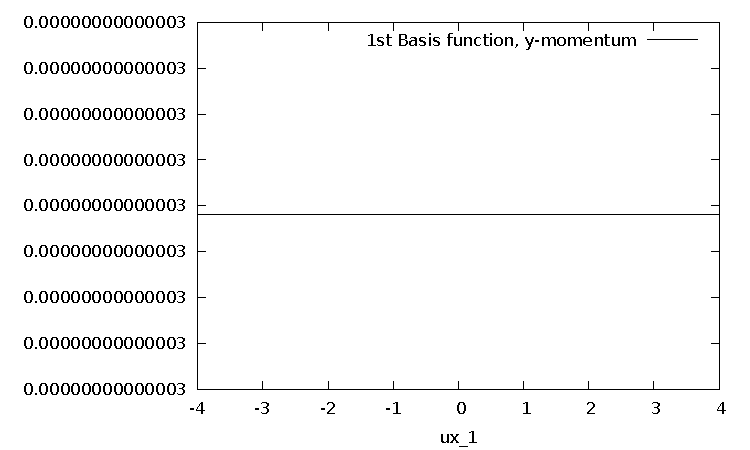
\includegraphics[scale=\zoomfactor]{{{ord2_varying_ux_1/10.0_10.0_10.0_10.0_10.0_10.0_y_0.0_0.0_0.0_0.0_0.0_0.0_0.0_0.0_0.0_0.0_0.0f01}}}
  % }
  \subfigure[2nd basis function, $x$-momentum] {
    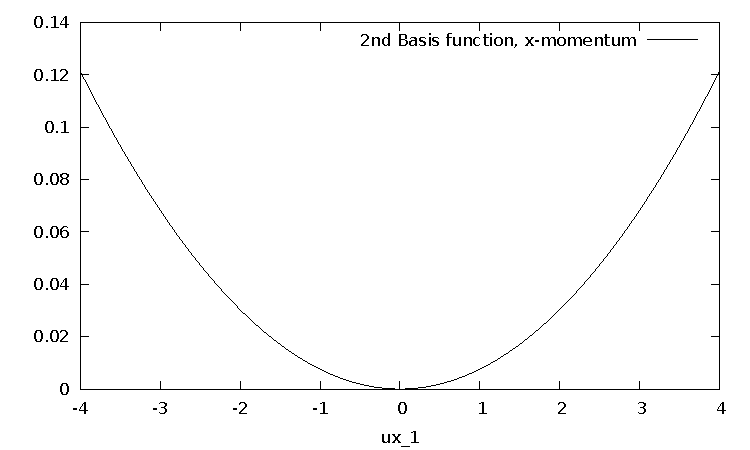
\includegraphics[scale=\zoomfactor]{{{ord2_varying_ux_1/10.0_10.0_10.0_10.0_10.0_10.0_y_0.0_0.0_0.0_0.0_0.0_0.0_0.0_0.0_0.0_0.0_0.0f02}}}
  }
  % \subfigure[] {
  %   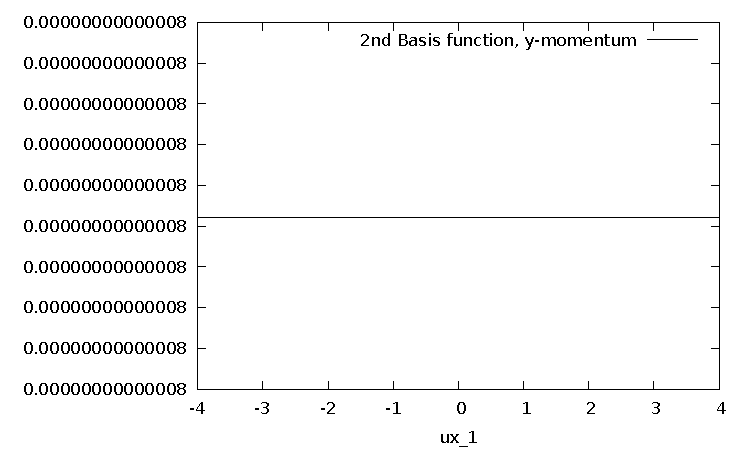
\includegraphics[scale=\zoomfactor]{{{ord2_varying_ux_1/10.0_10.0_10.0_10.0_10.0_10.0_y_0.0_0.0_0.0_0.0_0.0_0.0_0.0_0.0_0.0_0.0_0.0f03}}}
  % }
  \subfigure[3rd basis function, $x$-momentum] {
    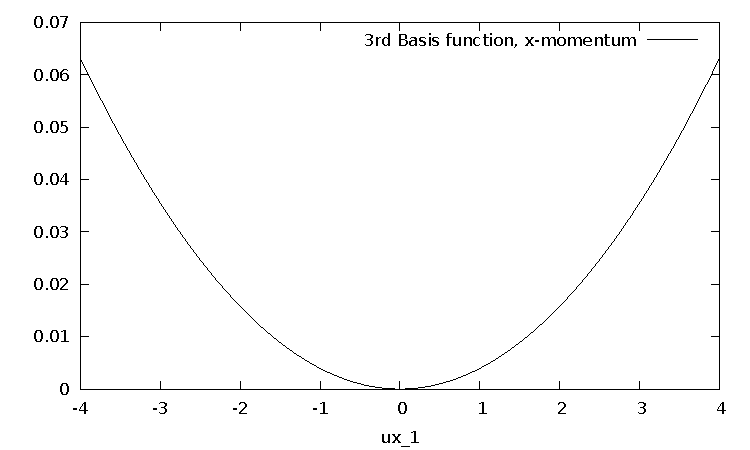
\includegraphics[scale=\zoomfactor]{{{ord2_varying_ux_1/10.0_10.0_10.0_10.0_10.0_10.0_y_0.0_0.0_0.0_0.0_0.0_0.0_0.0_0.0_0.0_0.0_0.0f04}}}
  }
  % \subfigure[] {
  %   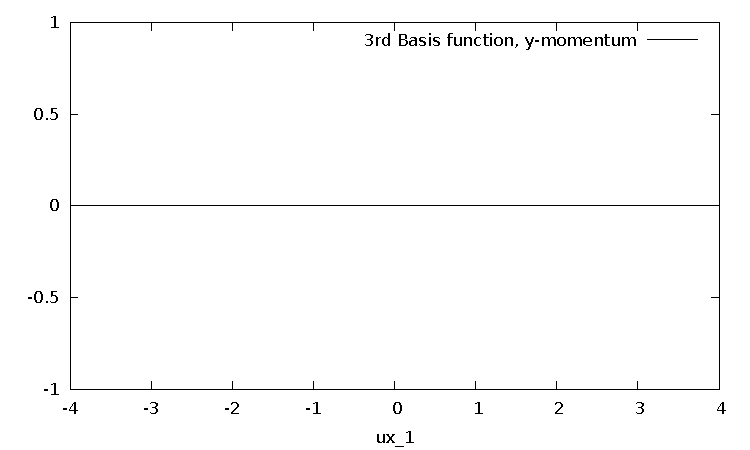
\includegraphics[scale=\zoomfactor]{{{ord2_varying_ux_1/10.0_10.0_10.0_10.0_10.0_10.0_y_0.0_0.0_0.0_0.0_0.0_0.0_0.0_0.0_0.0_0.0_0.0f05}}}
  % }
  \subfigure[4th basis function, $x$-momentum] {
    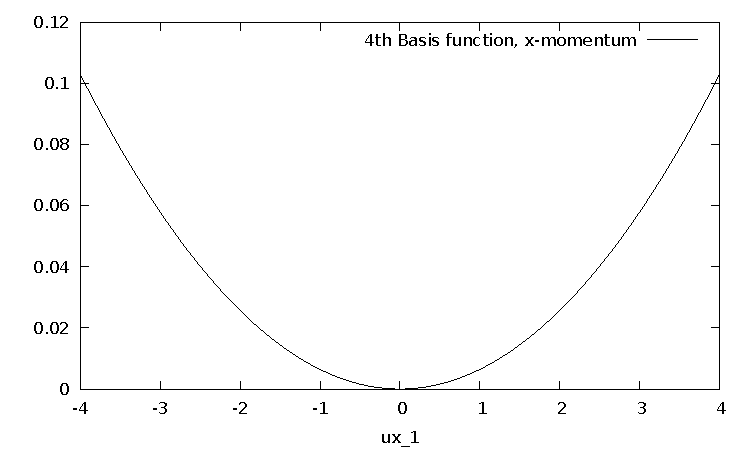
\includegraphics[scale=\zoomfactor]{{{ord2_varying_ux_1/10.0_10.0_10.0_10.0_10.0_10.0_y_0.0_0.0_0.0_0.0_0.0_0.0_0.0_0.0_0.0_0.0_0.0f06}}}
  }
  % \subfigure[] {
  %   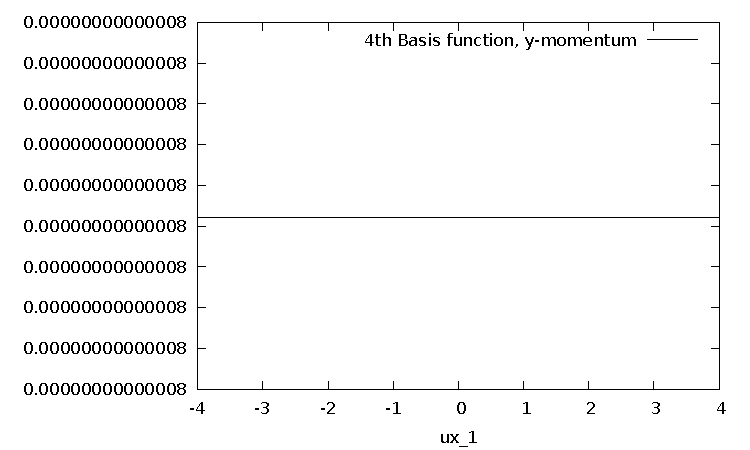
\includegraphics[scale=\zoomfactor]{{{ord2_varying_ux_1/10.0_10.0_10.0_10.0_10.0_10.0_y_0.0_0.0_0.0_0.0_0.0_0.0_0.0_0.0_0.0_0.0_0.0f07}}}
  % }
  \subfigure[5th basis function, $x$-momentum -- all $y$-momentum] {
    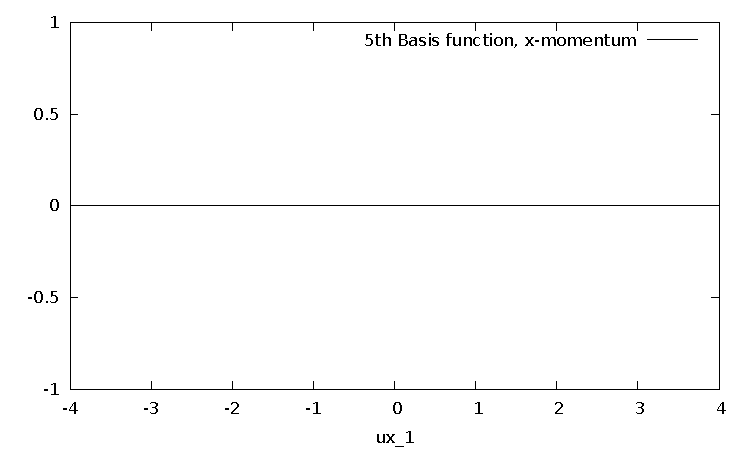
\includegraphics[scale=\zoomfactor]{{{ord2_varying_ux_1/10.0_10.0_10.0_10.0_10.0_10.0_y_0.0_0.0_0.0_0.0_0.0_0.0_0.0_0.0_0.0_0.0_0.0f08}}}
  }
  % \subfigure[] {
  %   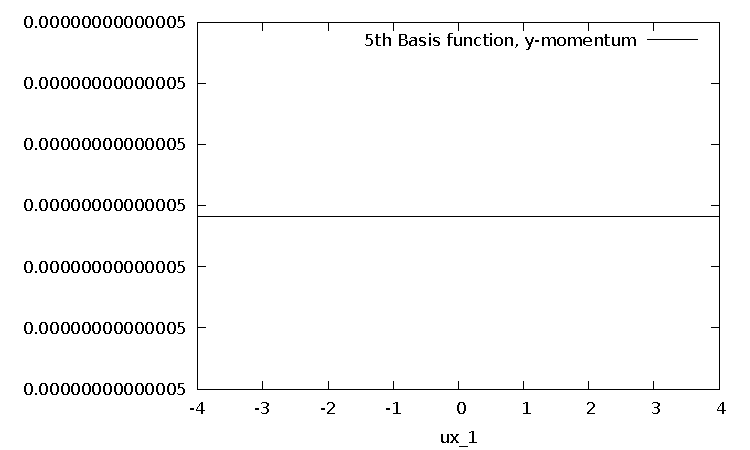
\includegraphics[scale=\zoomfactor]{{{ord2_varying_ux_1/10.0_10.0_10.0_10.0_10.0_10.0_y_0.0_0.0_0.0_0.0_0.0_0.0_0.0_0.0_0.0_0.0_0.0f09}}}
  % }
  \subfigure[6th basis function, $x$-momentum] {
    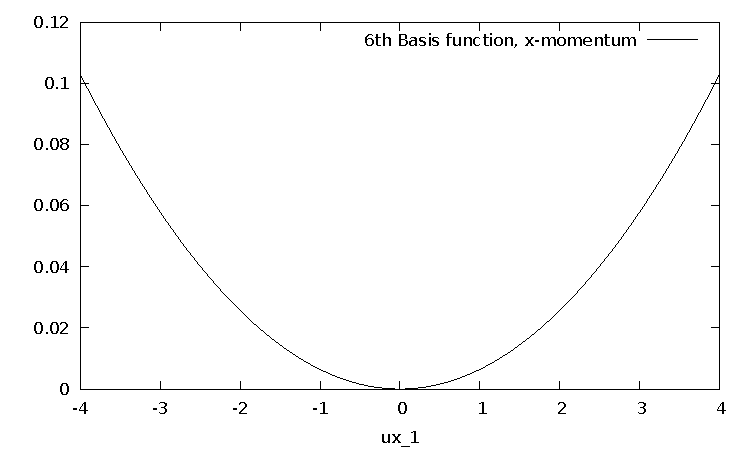
\includegraphics[scale=\zoomfactor]{{{ord2_varying_ux_1/10.0_10.0_10.0_10.0_10.0_10.0_y_0.0_0.0_0.0_0.0_0.0_0.0_0.0_0.0_0.0_0.0_0.0f10}}}
  }
  % \subfigure[] {
  %   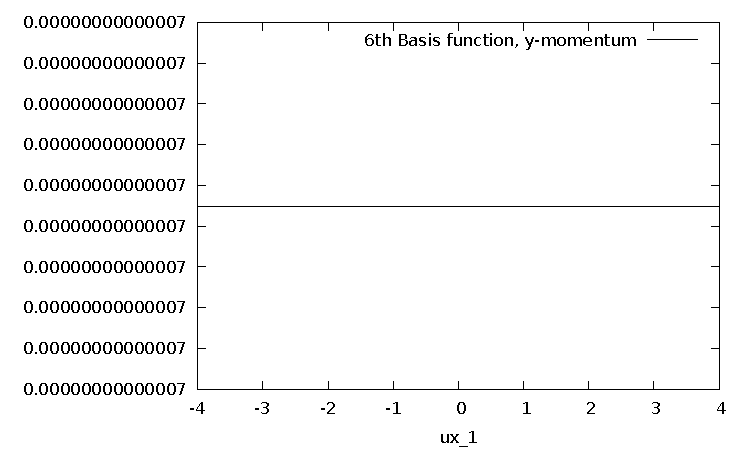
\includegraphics[scale=\zoomfactor]{{{ord2_varying_ux_1/10.0_10.0_10.0_10.0_10.0_10.0_y_0.0_0.0_0.0_0.0_0.0_0.0_0.0_0.0_0.0_0.0_0.0f11}}}
  % }
\caption{Error plots for varying $u_{x,1}$. All other momentums are set to 0 (i.e. $u_{x,2}=\dots=u_{x,6}=u_{y,1}=\dots=u_{y,6}=0$), all heights are set to 10 (i.e. $h_1=\dots=h_6=10$). The error is zero for \emph{all} $y$-momentums and for the $x$-momentum of the 5th basis function.}
\label{fig:ord2_varying_ux_1}
\end{figure}

%%% Local Variables:
%%% TeX-master: "../results.tex"
%%% End:
